%! Author = Philipp Emmenegger
%! Date = 30/06/2021

\section{Introduction}
\textbf{Artificial Intelligence}
\begin{itemize}
    \item broad concept
    \item different interpretations
    \item we do not have a definition of inteligence
\end{itemize}
\textbf{Statistical machine learning}
\begin{itemize}
    \item Algorithms and applications where computer learn from data
\end{itemize}
\textbf{AGI}
\begin{itemize}
    \item Artificial General Intelligence
    \item Hypothetical computer program that can perform intellectual tasks as well as, or better than a human.
\end{itemize}
\textbf{Turing Test}
\begin{itemize}
    \item Also called imitation game
    \item Tests of a machine's ability to exhibit intelligent behaviour equivalent to, or indistinguishable from that of a human
    \item Has some philosophical problems (Complex problems, humans cant solve / AI must learn to lie)
\end{itemize}
\textbf{Examples of application (today)}
\begin{itemize}
    \item Personalization of news feeds
    \item Product searching and recommendation s on eCommerce platforms
    \item Voice-to-text
    \item Predictive maintenance
\end{itemize}
\textbf{Bias}
\begin{itemize}
    \item Results that are systematically prejudiced due to faulty assumptions
    \item The inability for a machine learning method (like linear regression) to capture the true relationship, eg. Straight Line can't be curved like the true relationship
\end{itemize}
\textbf{Variance}
\begin{itemize}
    \item Difference of fits between data sets.\\
    \item The difference in fits between training and testing set (different data sets in general)
    \item \textcolor{blue}{Low variance} Sum of Squares are very similar for different datasets
\end{itemize}
The ideal ML algorithm has low bias and can accurately model the true relationship and it has low variability by producing consistent predictions across different datasets.

\subsection{Tasks and Algorithms of Machine Learning}
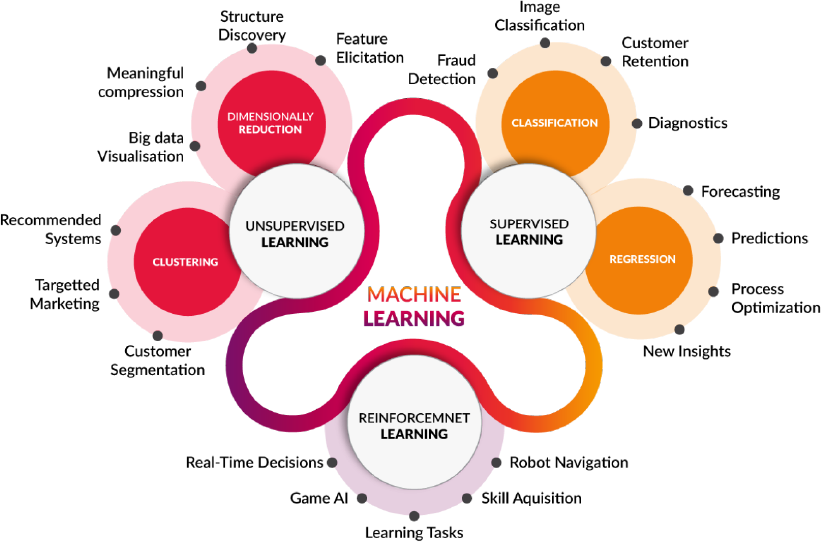
\includegraphics[width=\linewidth]{machine_learning_sections.png}

\subsection{Dialogflow}
\textbf{Intents}
An intent categorizes an end-user's intention for one conversation turn.
\begin{itemize}
    \item Recognizes the need of a user
    \item Require training to match to user inputs
    \item Follow up Intents (on Success)
    \item Fallback Intents (on Failure)
\end{itemize}
\textbf{Entities}
Each intent parameter has a type, called the entity type, which dictates exactly how data from an end-user expression is extracted.
\begin{itemize}
    \item Extract information from user inputs
    \item Help to identify required intent
    \item \textcolor{blue}{System Entities} Date and time / Numbers / Amounts / Units / etc.
    \item \textcolor{blue}{Developer Entities} defined by list of words (@pizza-type / @drink / etc.)
    \item \textcolor{blue}{User Entities} transient, temporary Information based on Conversation (@previous-orders)
\end{itemize}
\textbf{Dialog}
\begin{itemize}
    \item \textcolor{blue}{Linear} Gather a list of information
    \item \textcolor{blue}{Non Linear} Using Contexts
\end{itemize}
\textbf{Context}
\begin{itemize}
    \item Each Intent can have Input \& Output Context
    \item Intents are active based on active Context
    \item Expire automatically
\end{itemize}
\textbf{Fulfillment}
\begin{itemize}
    \item Action triggered on fullfilled Intents
    \item e.g. Webhook
\end{itemize}
\textbf{Predictive modeling} Train model for predictions \\
\textbf{Feature Engineering}
\begin{itemize}
    \item The process of identifying useful, additional input from the data
    \item A typical preprocessing step before the actual learning process starts
\end{itemize}
\textbf{Deep neural network} ANNs with multiple hidden layers \\

\textbf{Feature} e.g. Years of working experience, school grades

\subsection{7 Steps of Machine Learning}
\begin{enumerate}
    \item \textcolor{blue}{Gathering data} Collect quantity/quality data for training/testing
    \item \textcolor{blue}{Preparing that data} Cleanup data (remove duplicates, correct errors, deal with missing values, normalize data, convert data types)
    \item \textcolor{blue}{Choosing a model} Select the right algorithm(s)
    \item \textcolor{blue}{Training} Train the model, each iteration of process is a training step
    \item \textcolor{blue}{Evaluation} Use metrics to measure objective performance of the model, test model against previously unseen data, good train/eval split is 80/29, 70/30
    \item \textcolor{blue}{Hyperparameter tuning} Try to improve upon the positive results achieved during the evaluation through gamble with stepNumber of training steps, learning rate, initialization values and distribution
    \item \textcolor{blue}{Prediction} Model should be ready for practical applications
\end{enumerate}
